\section{Initialize repository}
\begin{itemize}
\item \code{git init .}, initialize a new repository in the current folder 
\item \code{git clone <repository url>} downloads a full remote repository to the local computer, but has to be done on an empty folder.
\end{itemize}

\section{Work with GIT}
\begin{itemize}
\item \code{git add <files>}, add some files to the staging area.  with "." add every file in the folder, "*.tex" just the \LaTeX  files.
\item \code{git status}, show the status of the repo (added files, untracked files, etc.
\item \code{git log}, gives information about all the commits of the repository, with each comment.
\item \code{git commit -m "message"}, Commits locally the changes. Files marked as ``to-be-committed`` using \code{git add} or \code{git rm} commands will be ''stored`` in the internal database. The commit description is specified with the \textbf{-m} param.
\item \code{git commit -am "message"}, commits all changed files (it's like a \\ \code{git add . \&\& git commit -m "message"}, using the specified message as commit description.
\\ \code{git reset HEAD <nome\ file>} to remove a file from the staging area 
\end{itemize}

\section{Remote repository management}
\begin{itemize}
\item \code{git fetch <repository name>}, update just the ``header'' of the repo, which contains the list of branches and so on.
\item \code{git remote add <repo name> <repo url>}, specify a remote repo url that will be used with \code{git push} or \code{git pull} commands. 
\item \code{git push -u <repo name> <branch name>} upload the changes to \code{repo_name} in the branch \code{branch_name}. \code{-u} means that (in future) typing \code{git push} will always use this host and branch.
\item \code{git pull <repo name> <branch name>} download the changes from the branch \code{branch_name} on \code{repo_name}. If the remote repo is stored as default (or it's the only one), \code{git pull} will work as well.
\end {itemize}

\section{Branch}
\subsection{Create a new Branch}
\begin{itemize}
\item \code{git checkout -b <new branch name>}
\item \code{git add <file to commit>}
\item \code{git commit -m "comment"}
\item \code{git push -u <repo name> <new branch name>}
\end{itemize}

\subsection{Merge Branch with master}
\begin{itemize}
\item \code{git checkout master}, move to the master branch (or whatever branch you want to merge with).
\item \code{git merge <branch name>}, merges the specified branch with the actual branch.
\end{itemize}

\subsection{Switch to an other branch}
\begin{itemize}
\item \code{git checkout <branch name>}
\end{itemize}

\section{Undo Commands}
\begin{itemize}
\item \code{git reset --soft}, unstage committed files
\item \code{git reset --hard}, delete changes to the last commit
\item \code{git commit --amend}, change last commit
\item \code{git revert <SHA-1 commit id>}, revert to a specific commit
\end{itemize}

Just a note, \code{git commit --amend} will change the whole GIT tree. So, 
if the commit is already uploaded on  the server, a \code{git push -f} will be
required.  \code{git push -f} is the second name of Satan. Be aware that
after that there will be high chances to destroy the whole GIT tree, losing
everything. Hence, \code{git commit --amend} is bad.

\section{Useful links}
\begin{itemize}
\item \url{https://try.github.com}
\end{itemize}

\begin{figure}[h]
	\centering
	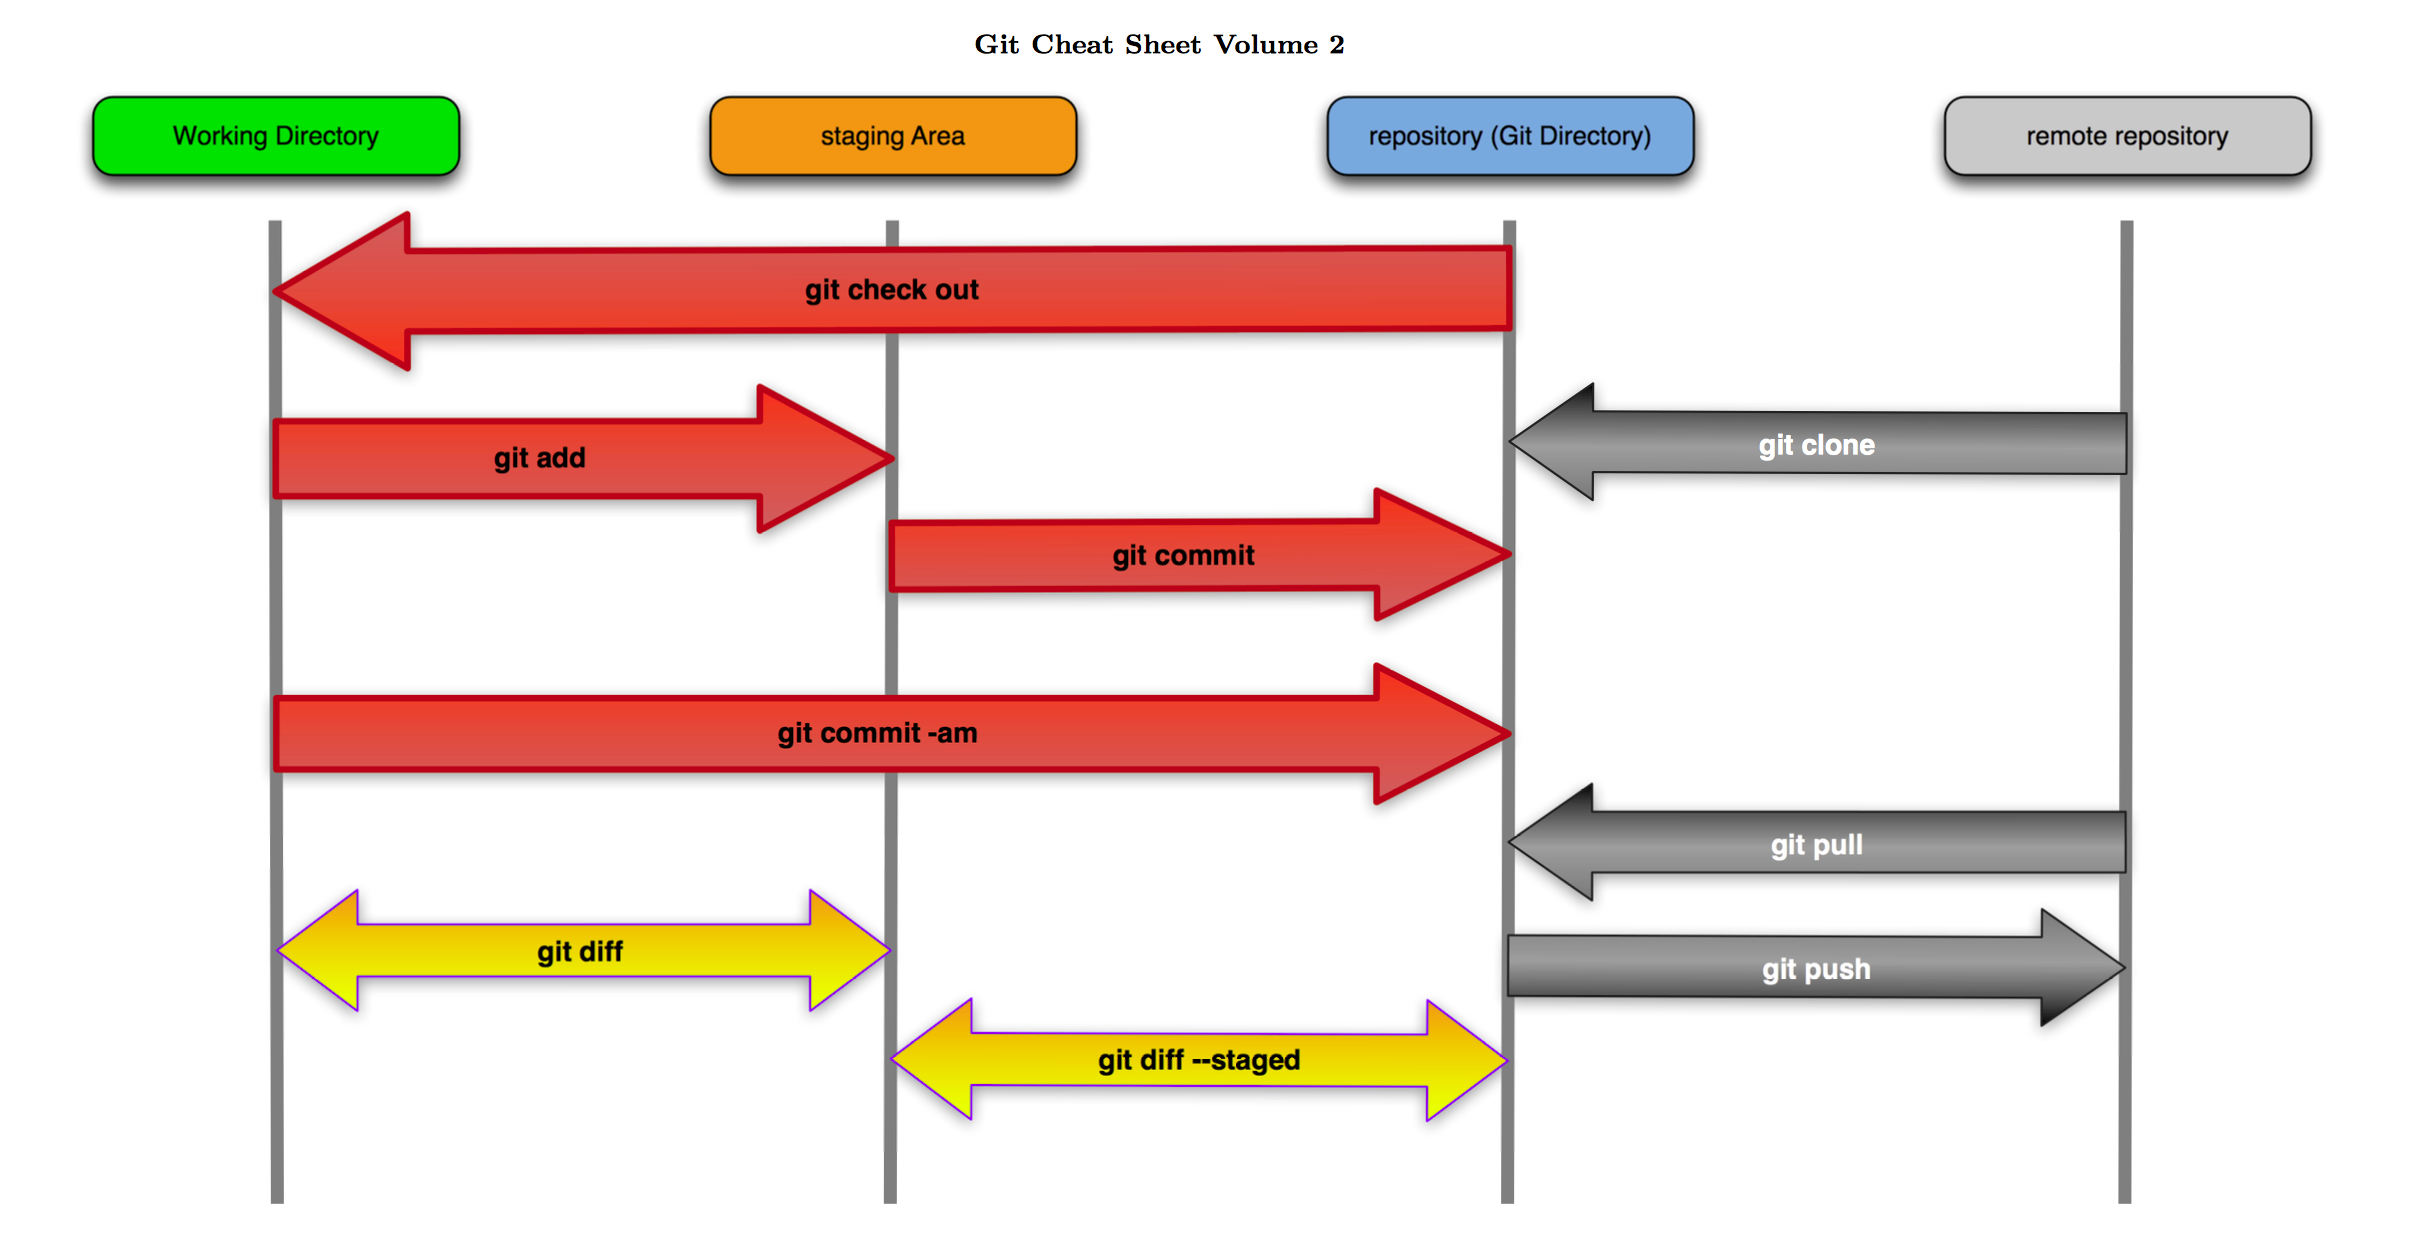
\includegraphics[width=\textwidth]{gfx/git_graph}
	
	\caption{Comandi GIT}
	\label{Fig:Commands}
\end{figure}